\documentclass[../practica_09.tex]{subfiles}

\begin{document}

    \begin{enumerate}
        \item $ \int_{\frac{\pi}{4}}^{\frac{3\pi}{4}} \int_1^2 r dr d\theta $

            $ D = \{(x,y,z) \in \mathbb{R}^3:$
                \begin{itemize}
                    \item $\frac{\pi}{4} \leq \theta \leq \frac{3\pi}{4}$
                    \item $1 \leq r \leq 2$
                \end{itemize} 
                $\}$

            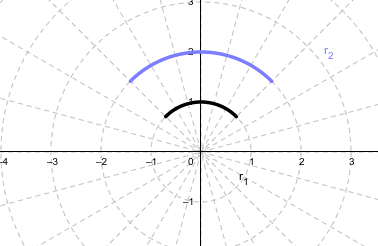
\includegraphics[scale=0.8]{ej01/resources/ej01.png}

            \begin{itemize}
                \item $\int_1^2 r dr = $
                
                    $ \left. \frac{r^2}{2} \right |_1^2 = $

                    $ 2 - \frac{1}{2} = \frac{3}{2} $

                \item $ \int_{\frac{\pi}{4}}^{\frac{3\pi}{4}} \frac{3}{2} d\theta = $
                
                $\left. \frac{3\theta}{2} \right |_{\frac{\pi}{4}}^{\frac{3\pi}{4}} = $

                $ \frac{9\pi}{8} - \frac{3\pi}{8} =  $

                $ \frac{6\pi}{8} = \frac{3\pi}{4}$

            \end{itemize}

        \item $ \int_{\frac{\pi}{2}}^{\pi} \int_0^{2\sin(\theta)} r dr d\theta$

            $ D = \{(x,y,z) \in \mathbb{R}^3: $
                \begin{itemize}
                    \item $0 \leq r \leq 2\sin(\theta)$
                    \item $\frac{\pi}{2} \leq \theta \leq \pi$
                \end{itemize}
                $\}$

            Media circunferencia con centro en $(1,1)$

            \begin{itemize}
                \item $\int_0^{2\sin(\theta)} r dr = $
                
                    $ \left. \frac{r^2}{2} \right |_0^{2\sin(\theta)} = $

                    $ 2\sin^2(\theta) $

                \item $2 \int_{\frac{\pi}{2}}^{\pi} \sin^2(\theta) d\theta = $
                
                    $ \left. \theta  \right |_{\frac{\pi}{2}}^{\pi} = $

                    $ \frac{\pi}{2} $

            \end{itemize}

    \end{enumerate}

\end{document}
